\chapter{Metodologia}
\label{sec:Metodologia}

Neste capítulo serão apresentados os métodos, ferramentas e o processo definido
para aplicação no presente trabalho visando alcançar o seu objetivo final.

  As seções estão dispostas em:

  \begin{enumerate}
    \item \textbf{Metodologia de Desenvolvimento} Descrição do fluxo que será
    adotado para análise dos fatores pertinentes ao escopo do presente trabalho.
    \item \textbf{Tecnologias e ferramentas} Breve descrição das tecnologias,
    que serão utilizados.
  \end{enumerate}

\section{Metodologia de Desenvolvimento}

Pretende-se com este trabalho realizar um estudo de caso acerca do desenvolvimento
de software na empresa Rua Dois, considerando os aspectos que são pertinentes para
uma \textit{startup}. Para tal, será realizada uma comparação entre duas arquiteturas
de software distintas adotadas dentro da Rua Dois para um mesmo sistema. Ao final,
com os resultados obtidos desta comparação e com base em estudos realizados por meio
de pesquisa exploratória pretende-se elencar boas práticas e recomendações para o
desenvolvimento de software na empresa. Dessa forma, esta seção visa descrever
os objetos de análise, os aspectos a serem considerados na análise comparativa e
como se dará a análise final.

\subsection{Objetos de análise}

O desenvolvimento do sistema da Rua Dois foi marcado por duas fases distintas.
Estas fases serão abordadas na \autoref{sec:ArquiteturaDoSistema} e serão
os objetos de análise do presente trabalho para a realização da análise
comparativa. A seguir é apresentada uma breve descrição sobre cada fase:

    \begin{description}
        \item [Fase 1] Fase inicial de desenvolvimento do software da Rua Dois,
        marcado por uma arquitetura de microsserviços e constantes alterações
        no software visando validar ideias.
        \item [Fase 2] Segunda fase de desenvolvimento do software da Rua Dois,
        marcado por uma arquitetura monolítica e um escopo melhor definido.
    \end{description}

\subsection{Etapas do desenvolvimento}

O desenvolvimento do presente trabalho acontecerá nas seguintes etapas:

    \begin{description}
        \item[Etapa 1] Estudo acerca da arquitetura adotada em cada fase;
        \item[Etapa 2] Coleta e levantamento de dados pertinentes aos aspectos que serão
        considerados para realização da análise comparativa;
        \item[Etapa 3] Análise comparativa entre os dados coletados;
        \item[Etapa 4] Definição de diretrizes acerca do desenvolvimento de software
        escalável na Rua Dois.
    \end{description}

A seguir segue a descrição de cada etapa.

\subsubsection{Etapa 1: Estudo acerca das arquiteturas adotadas}

Pretende-se nesta etapa descrever os elementos arquiteturais adotados em cada fase,
quais tecnologias foram utilizadas, quais as dificuldades encontradas e o contexto
da empresa e suas respectivas fases.

\subsubsection{Etapa 2: Coleta e levantamento de dados}
\label{sec:Etapa2}

Para os objetos de análise definidos serão levantados os seguintes dados e informações
julgados como pertinentes para a análise final:

    \begin{description}
        \item [Qualidade de código] Usando métricas de qualidade de código pretende-se
        avaliar questões referentes a coesão e acoplamento do sistema em cada uma das
        fases.
        \item [Práticas de desenvolvimento de Software] Elencar quais práticas de
        desenvolvimento de software foram aplicadas em cada fase e como estas práticas
        afetaram a qualidade do sistema em questão.
        \item [Nível de conhecimento e experiência da equipe no contexto de \textit{startups}]
        Aplicação de um questionário entre os membros do time de desenvolvimento participantes
        de cada fase, com o intuito de avaliar o domínio do time com as tecnologias utilizadas
        e a experiência com desenvolvimento de software dentro de \textit{startups}.
        \item [Tecnologias utilizadas] Identificar quais foram as tecnologias utilizadas em
        cada fase, como elas influenciaram o desenvolvimento e qual a escalabilidade de cada
        tecnologia.
        \item [Escalabilidade do sistema] Por meio de testes de escalabilidade, coletar
        informações sobre o nível de escalabilidade da arquitetura adotada em cada fase.
        \item [Relação com o ciclo de vida de uma \textit{startup}] Avaliar qual foi o
        contexto de desenvolvimento com base nas fases de uma \textit{startup} e como a
        arquitetura adotada influenciou nesse contexto.
    \end{description}

Para cada um dos itens definidos sera executado o processo ilustrado na
\autoref{fig:ProcessoAnaliseComparativa} com o propósito de definir os métodos utilizados
e coletar os dados.

    \begin{figure}[h]
      \caption{Processo para realização da coleta de dados\label{fig:ProcessoAnaliseComparativa}}
      \centering
      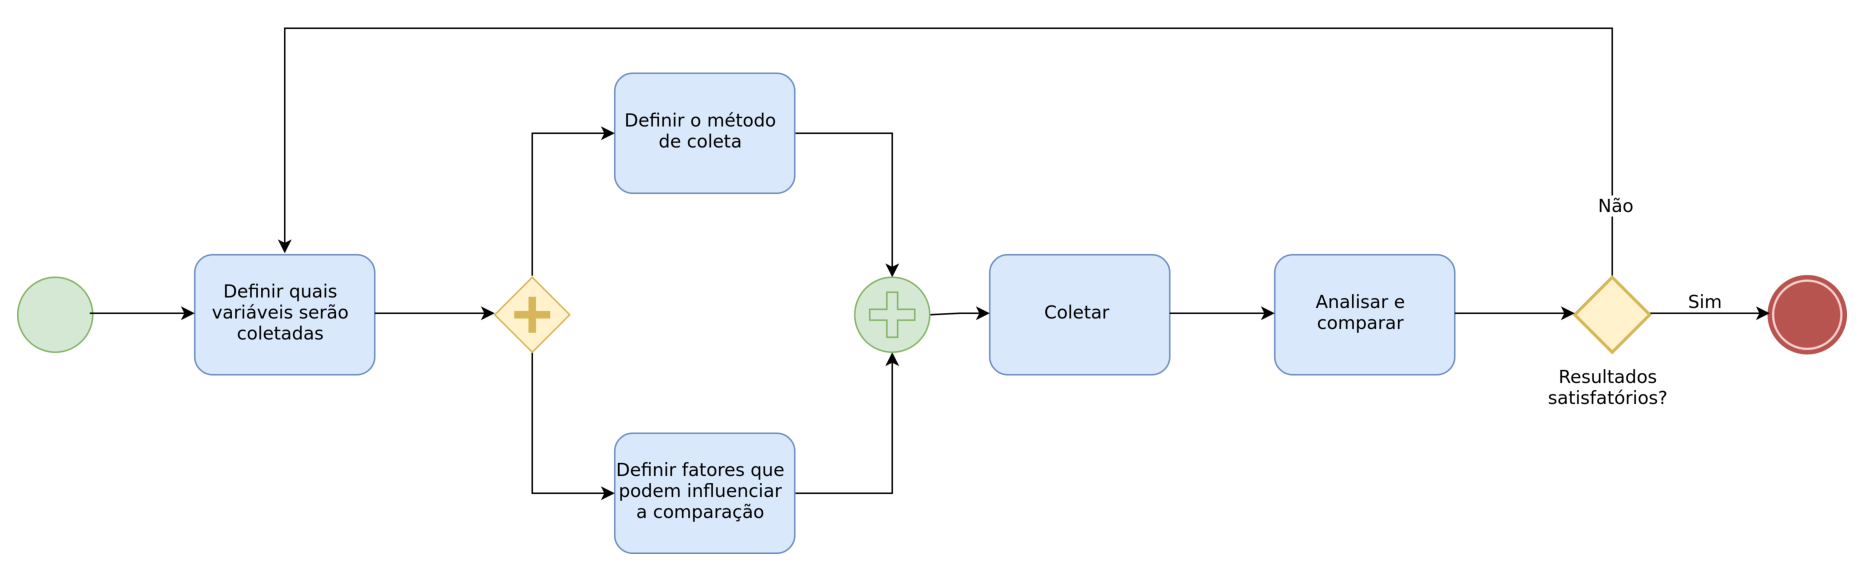
\includegraphics[keepaspectratio=true,scale=0.5]{figuras/metodologiaAnalise.eps}
    \end{figure}

\subsubsection{Etapa 3: Análise comparativa}

Uma vez coletado os dados da etapa anterior, pretende-se fazer uma análise comparativa
entre as fases definidas como objeto de estudo, visando alinhar as diferenças de
escalabilidade e de desenvolvimento referentes a cada uma.

\subsubsection{Etapa 4: Definição das diretrizes}

Com base na análise comparativa realizada e em uma pesquisa exploratória acerca de
desenvolvimento de software escalável, pretende-se elaborar diretrizes para alcançar
um desenvolvimento sustentável e escalável dentro da Rua Dois, elencando possíveis
medidas a serem tomadas dentro da empresa para tal.


\section{Ferramentas}

As ferramentas que pretende-se usar para a execução deste trabalho são:

\begin{description}
    \item[Artillery] conjunto de ferramentas \textit{open source} escritas em Node.js
    para a realização de testes de carga em servidores. Permite simular vários usuários
    e avaliar fatores como a latência na resposta do servidor.
    \item[CloudWatch] serviço de monitoramento da Amazon que fornece dados e
    \textit{insights} para acompanhar as aplicações. Atualmente já é utilizado na
    Rua Dois e possui o registro de \textit{logs} desde o início da \textit{startup}.
    \item[Draw.io] editor gráfico online que permite a construção de processos e
    desenhos relevantes ao conteúdo apresentado.
    \item[Google Forms] ferramenta para aplicação de questionários e enquetes
    e organização dos resultados para análise. Visa-se utilizá-la para coleta
    de informações referentes aos conhecimento do time de desenvolvimento da Rua Dois.
    \item[Google Planilhas] ferramenta para construção de tabelas e gráficos.
    A qual pretende-se usar para realizar análises sobre os dados coletados.
\end{description}

